\chapter{Entwurf und Design}
\section{\acs{FPGA}-Design}
Nach Festlegung der Anforderungen wurde mit der Konzeption und Entwurfsphase des Gesamtsystemes sowie des \acs{FPGA}-Designs begonnen.

Hierbei wurde zuerst, anhand der Anforderungen, die Architektur des zu erstellenden FPGA-Designs festgelegt.

Die Kommunikation zwischen den einzelnen Modulen, besonders für den Datenaustausch, soll zum größten Teil mit einer \acs{AXI}-Stream basierten 
Schnittstelle umgesetzt werden. Für die, hauptsächlich zur Steuerung verwendete, Kommunikation zwischen \acs{FPGA}-Design und Rechenkern sollen
\acs{AXI}-Lite basierte Registerbänke verwendet werden.

In dem folgenden Entwurf nicht betrachtet werden die weiterhin notwendigen \acs{AXI}-Infrastruktur Blöcke, welche für die Kommunikation mit dem Rechenkern weiterhin benötigt werden.
Diese Blöcke werden jedoch aus Zeit- und Komplexitätsgründen nicht selbst umgesetzt. 
Eine hierarchische Gesamtübersicht des Designs ,mit \acs{AXI}-Infrastruktur, kann im Kapitel \ref{Chap:Impl} gefunden werden.

Als Architektur für den Funkempfangsteil des Designs wurde eine klassische \acs{QPSK}-Empfängerarchitektur mit direkter digitaler Abwärtsmischung gewählt.

\begin{figure}[h]
	\centering
	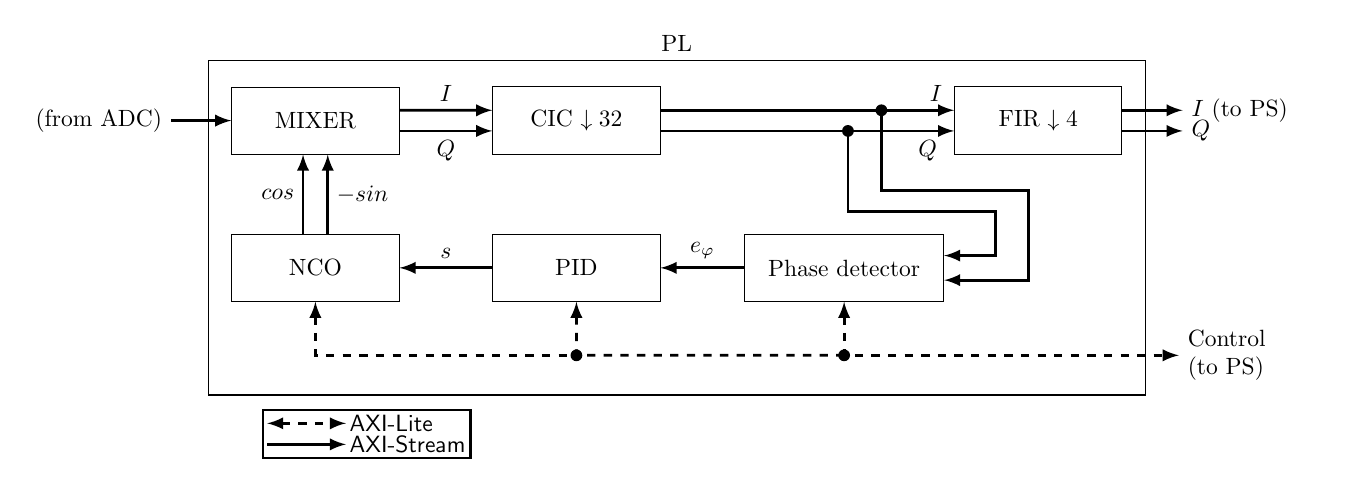
\begin{tikzpicture}[scale=0.85, every node/.style={scale=0.85}]
		\def\arow{7.0}
		\def\aarow{1.6}
		\def\abrow{5.5}
		\def\acrow{9.5}
		\def\adrow{12.4}
			
		\tikzset{
			basic/.style={rectangle,draw=black, top color=white,text centered},
			PLnode/.style={basic, inner sep=1em,minimum width=14cm, minimum height=5.0cm},	
			smallnode/.style={basic, inner sep=1em,minimum width=2.5cm, minimum height=1cm},
			branch/.style={fill,circle,minimum size=5pt,inner sep=0pt,outer sep=-1pt},
			sarrow/.style={->, >={latex}, line width=1.0pt},
    		carrow/.style={<->, >={latex}, dashed, line width=1.0pt}
 		}
 		
 		\node[PLnode, label=above:PL] (PL) at (\arow,1.5) {};

		% internal Nodes

 		\node[smallnode] (PL_NCO)   at (\aarow,0.9) {NCO};
	 	\node[smallnode] (PL_MIX) at (\aarow,3.1) {MIXER}; 		 
 		\node[smallnode] (PL_CIC) at (\abrow,3.1) {CIC $\downarrow 32$};
 		\node[smallnode] (PL_FIR) at (\adrow,3.1) {FIR $\downarrow 4$};
 		\node[smallnode] (PL_PID) at (\abrow,0.9) {PID};
 		\node[smallnode] (PL_PD) at  (\acrow,0.9) {Phase detector};

		% internal interconnect arrows

 		\draw[sarrow, ->] (PL_NCO.70) -- (PL_MIX.-70) node[midway,right] {$-sin$};
 		\draw[sarrow, ->] (PL_NCO.110) -- (PL_MIX.-110) node[midway,left] {$cos$};

 		\draw[sarrow, ->] (PL_MIX.7)  -- (PL_CIC.173) node[midway,above] {$I$};
 		\draw[sarrow, ->] (PL_MIX.-7) -- (PL_CIC.-173) node[midway,below] {$Q$};
	 	
	 	\draw[sarrow, ->] (PL_CIC.7)  -- ++(3.3,0) node[branch](bI){} -- (PL_FIR.173) node[near end, above] {$I$};
 		\draw[sarrow, ->] (PL_CIC.-7) -- ++(2.8,0) node[branch](bQ){} -- (PL_FIR.-173) node[near end, below] {$Q$};

 		\draw[sarrow, ->] (PL_PID.west)  -- (PL_NCO.east) node[midway,above] {$s$}; 		
 		\draw[sarrow, ->] (PL_PD.west)  -- (PL_PID.east) node[midway,above] {$e_\varphi$}; 		
 		
 		\draw[sarrow, ->] (bI)  |- ++(2.2, -1.2) |- (PL_PD.-7); 	
 		\draw[sarrow, ->] (bQ)  |- ++(2.2, -1.2) |- (PL_PD.7); 	

		% control connections
		
		\draw[carrow, <->] (PL_PD.south)  -- ++(0, -0.8) node[branch](bC0){} -- ++(5,0) node[right,text width=2cm]{Control\\(to PS)}; 
		\draw[carrow, <-] (PL_PID.south)  -- ++(0, -0.8) node[branch](bC1){} -- (bC0);
 		\draw[carrow, <-] (PL_NCO.south)  |- (bC1);
 		
 		% external connections
 		\draw[sarrow, ->] (PL_FIR.7)  -- ++(0.9,0) node[right] {$I$ (to PS)};
 		\draw[sarrow, ->] (PL_FIR.-7) -- ++(0.9,0) node[right] {$Q$};
 		\draw[sarrow, <-] (PL_MIX.west) -- ++(-0.9,0) node[left] {(from ADC)};
 		
 		% legend
 		\path ([xshift=35mm,yshift=-2mm]current bounding box.south west) node[matrix,anchor=north west,cells={nodes={font=\sffamily,anchor=west}}, draw,thick,inner sep=1pt]{
  			\draw[carrow](0,0) -- ++ (1,0); & \node{AXI-Lite};\\
  			\draw[sarrow](0,0) -- ++ (1,0); & \node{AXI-Stream};\\
 		};
	\end{tikzpicture}
	\caption{Architektur des \acs{FPGA}-Designs (ohne \acs{AXI}-Infrastruktur)}
\end{figure}

Die Hauptkomponenten des \acs{FPGA}-Designs werden in den folgenden Abschnitten näher erklärt.

\subsection{Mischer (Mixer)}
Der Mischer hat die Aufgabe den von dem \acs{ADC} abgetasteten Datenstrom mit den, vom lokalen Oszillator erzeugten, Trägern zu multiplizieren und so das Nutzsignal in das
Basisband zu verschieben. Die besondere Schwierigkeit liegt hier dabei, dass der Mischer mit der Taktrate des \acs{ADC}s $f_{ADC}$ betrieben werden muss.

Für den Empfang von \acs{QPSK}-modulierten Daten, ist es notwendig einen komplexen Mischer \textit{(sogenannter I/Q-Mischer)} zu verwenden.
Als Eingang dienen zwei vom lokalen Oszillator (\acs{NCO}) erzeugten Referenzsignale \textit{(Trägersignale)}, sowie der \acs{ADC}-Datenstrom ($x[n]$),
welche dann wie folgt Multipliziert werden: 
\begin{equation}
	I[n] = x[n]\cdot cos(2\pi\frac{f}{f_{ADC}}\cdot n) 
\end{equation}
\begin{equation}
	Q[n] = x[n]\cdot -sin(2\pi\frac{f}{f_{ADC}}\cdot n) 
\end{equation}

Es entsteht ein komplexer Datenstrom welcher dann für die weitere Verarbeitung genutzt werden kann:
\begin{equation}
	\underline{y}[n] = I[n] - j \cdot Q[n] = x[n]\cdot e^{j2\pi\frac{f}{f_{ADC}}\cdot n}
\end{equation}

Durch die reale Natur des Eingangssignales entsteht bei der Mischung, zusätzlich zu dem komplexen Basisbandsignal, auch immer eine Signalkopie bei dem doppelten der Trägerfrequenz.
\cite{WPI_COSTAS}
Die nicht erwünschte Kopie, bei doppelter Trägerfrequenz, wird anschließend durch die Verwendung eines Tiefpassfilters eliminiert. 
Diese Aufgabe übernimmt hier der \acs{CIC}-Dezimierungsfilter.

Ein- und Ausgabeschnittstellen des Mischers sollen als \acs{AXI}-Stream Schnittstelle realisiert werden, wobei es notwendig ist jeden Taktzyklus einen neuen Datenwert
im Mischer zu verarbeiten. 

\subsection{Lokaler Oszillator (\acs{NCO})} \label{Sec:NCO}
Der lokale Oszillator hat die Aufgabe die von dem Mischer verwendeten lokalen Referenzsignale zu erzeugen.
Die Frequenz der erzeugten Schwingungen wird hierbei extern, durch Rechenkern oder Phasenregelschleife, vorgegeben. 

Umgesetzt ist der lokale Oszillator als Numerisch gesteuerter Oszillator (\acs{NCO}). 
Die notwendigen Sinus-/Kosinus-Ausgangssignale werden hierbei durch die sogenannte direkte digitale Synthese (\acs{DDS}) erzeugt.

Dabei handelt es sich effektiv um einen Zähler (Phasen-Akkumulator, $n$-Bit breit) von welchem anschließend die untersten $m$-Bit verwendet werden
um die Ausgangsdatenwerte in einer Lookup-Tabelle nachzuschlagen.
Anhand der Schrittweite $s$ um welche der Phasen-Akkumulator jeden Taktzyklus erhöht wird lässt sich die Grundfrequenz der ausgegebenen Sinusschwingungen einstellen.

\begin{figure}[h]
	\centering
	\begin{tikzpicture}[scale=0.85, every node/.style={scale=0.85}]
		\def\arow{0.0}
		\def\brow{4.0}
		\def\crow{10.0}
			
		\tikzset{
			basic/.style={rectangle,draw=black, top color=white,text centered},
			smallnode/.style={basic, inner sep=1em,minimum width=2.5cm, minimum height=1cm},
			branch/.style={fill,circle,minimum size=5pt,inner sep=0pt,outer sep=-1pt},
			sarrow/.style={->, >={latex}, line width=1.0pt},
    		carrow/.style={<->, >={latex}, dashed},
    		buswidth/.style={decoration={ markings,
  				mark= at position 0.5 with {\node[font=\footnotesize] {/};\node[below=1pt] {\tiny #1};}
  			}, postaction={decorate}}
 		}

		% Komponenten 		
 		
 		\node[circle, draw=black, fill=white] (SUM) at (\arow,0) {$\Sigma$};	
 		\node[smallnode] (ACC) at (\brow, 0) { Phasen-Akkumulator };
 		\node[smallnode, text width=2cm] (SLUT) at (\crow, 0) { Lookup-Tabelle\\$-sin(\varphi)$ };
 		\node[smallnode, text width=2cm] (CLUT) at (\crow, -2.5cm) { Lookup-Tabelle\\$cos(\varphi)$ };

		% Interne Verbindungen

		\draw[sarrow, ->, buswidth={n}] (SUM.east) -- (ACC.west);
		\draw[sarrow, ->, buswidth={m}] (ACC.east) -- ++(0.5,0) node[branch](b0){} -- (SLUT.west);
		\draw[sarrow, -] (b0) -- ++(0,-2) node(b1){};
		\draw[sarrow, ->, buswidth={m}] (b1.north) |- (CLUT.west);
		\draw[sarrow, ->, buswidth={n}] (b0) -- ++(0,1) -- ++(-1,0) -| (SUM.north);

		% Ausgänge
		
		\draw[sarrow, <-, buswidth={n}] (SUM.west) -- ++(-1,0) node[left]{Stellwert $s$};
		\draw[sarrow, ->] (SLUT.east) -- ++(1,0) node[right, text width=3cm]{$-sin(2\pi\frac{f}{f_{ADC}}\cdot n)$};
		\draw[sarrow, ->] (CLUT.east) -- ++(1,0) node[right, text width=3cm]{$cos(2\pi\frac{f}{f_{ADC}}\cdot n)$};
 		
	\end{tikzpicture}
	\caption{Schematischer Aufbau des lokalen Oszillators.}
\end{figure}

Die Breite des Phasen-Akkumulators, die Ausgangswertbreite und die Anzahl der Stützpunkte der Lookup-Tabelle haben einen großen Einfluss auf die Güte der erzeugten Schwingung.
\cite{IEEE_ART_DDS}

Der Zusammenhang zwischen Frequenzstellwert $s$ und der Ausgangsfrequenz der erzeugten Sinusschwingung $\frac{f}{f_{ADC}}$ ist abhängig von der Akkumulator-Bit-Breite $n$:
\begin{equation}
	\frac{f}{f_{ADC}} = \frac{s}{2^n}
\end{equation}

\subsection{\acs{CIC}-Dezimierungsfilter} \label{Sec:CIC}
Nach dem Mischen des Eingangssignales ist es für die weitere Verarbeitung notwendig, die Datenrate des gemischten Signales auf ein beherrschbares Maß zu reduzieren.
Vor der Datenreduktion ist es jedoch notwendig die Bandbreite des Signales auf ein adäquates Maß zu beschränken.
Zusätzlich dazu ist es notwendig das zweite Mischprodukt, bei doppelter Trägerfrequenz, von dem Nutzsignal im Basisband zu trennen.

Beide diese Aufgaben werden von einem Tiefpassfilter, hier als \acs{CIC}-Filter ausgeführt, übernommen.

Bei einem \acl{CIC}-Filter handelt es sich grundsätzlich um einen \acs{FIR}-Mittelwertfilter.

\begin{figure}[h]
	\centering
	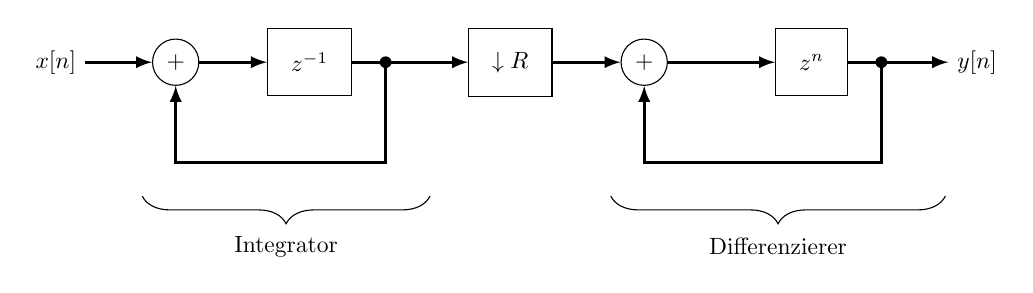
\begin{tikzpicture}[scale=0.85, every node/.style={scale=0.85}]
		\def\arow{0.0}
		\def\brow{-2.0}
			
		\tikzset{
			basic/.style={rectangle,draw=black, top color=white,text centered},
			smallnode/.style={basic, inner sep=1em,minimum width=1cm, minimum height=1cm},
			branch/.style={fill,circle,minimum size=5pt,inner sep=0pt,outer sep=-1pt},
			sarrow/.style={->, >={latex}, line width=1.0pt},
    		carrow/.style={<->, >={latex}, dashed},
    		buswidth/.style={decoration={ markings,
  				mark= at position 0.5 with {\node[font=\footnotesize] {/};\node[below=1pt] {\tiny #1};}
  			}, postaction={decorate}}
 		}

		% Komponenten 		
 		
 		\node[circle, draw=black, fill=white] (ISUM) at (0,\arow) {$+$};
 		\node[smallnode] (IDELAY) at (2,\arow) {$z^{-1}$};
 		\node[smallnode] (RATE) at (5,\arow) {$\downarrow R$};
 		
 		\node[circle, draw=black, fill=white] (DSUM) at (7,\arow) {$+$};
 		\node[smallnode] (DDELAY) at (9.5,\arow) {$z^{n}$};

		% Verbindungen Integratoren
	
 		\draw[sarrow, <-] (ISUM.west) -- ++(-1,0) node[left]{$x[n]$}; 		
 		\draw[sarrow, ->] (ISUM.east) -- (IDELAY.west);
 		\draw[sarrow, ->] (IDELAY.east) -- ++(0.5,0) node[branch](bI0){} |- ++(-1, -1.5) -| (ISUM.south);
 		\draw[sarrow, ->] (bI0) -- (RATE.west);
 		
 		% Verbindungen Differenzierer
	
 		\draw[sarrow, ->] (RATE.east) -- (DSUM.west); 		
 		\draw[sarrow, ->] (DSUM.east) -- (DDELAY.west);
 		\draw[sarrow, ->] (DDELAY.east) -- ++(0.5,0) node[branch](bD0){} |- ++(-1, -1.5) -| (DSUM.south);
 		\draw[sarrow, ->] (bD0) -- ++(1,0) node[right]{$y[n]$};		
 		
 		\draw [decorate,decoration={brace,amplitude=10pt,mirror}](-0.5,-2) -- (3.8,-2) node [black,midway,yshift=-0.75cm]{Integrator};
 		\draw [decorate,decoration={brace,amplitude=10pt,mirror}](6.5,-2) -- (11.5,-2) node [black,midway,yshift=-0.75cm]{Differenzierer};
	\end{tikzpicture}
	
	\caption{Struktur eines (transponierten) CIC-Filters 1. Ordnung}\cite{DSPREL_CIC}
\end{figure}

Diese Filterstruktur zeichnet sich, besonders bei hohen Taktraten und großen Dezimierungsverhältnissen, jedoch durch eine besonders effiziente Implementierung aus, 
da lediglich Subtraktionen und Additionen für die Umsetzung benötigt werden.

Nachteilig hierbei ist jedoch das nur bedingt steuerbare Frequenzverhalten des Filters welche sich grundsätzlich nur durch die Anzahl der Filterstufen (Ordnung $N$), 
das Dezimierungsverhältniss $R$ und die Anzahl der Verzögerungsstufen $D$ der Differenzierer steuern lässt. Wobei, anders als bei einem \acs{FIR}-Filter, nicht jedes beliebige
Frequenzverhalten des Filters erreicht werden kann.\cite{DSPREL_CIC}

Um das erreichen der notwendigen Taktfrequenz während der Implementierung des Filters zu vereinfachen soll der CIC-Filter in der transponierten Form umgesetzt werden.
Dies erlaubt die Verkürzung der kritischen Pfade durch die Nutzung der Verzögerungsregister als Pipelining-Register. Es können folglich einfacher höhere Taktraten erreicht werden.

Die notwendigen Filterparameter $R$ und $N$ sollen über generische Parameter während der Erzeugung des \acs{FPGA}-Bitstreams eingestellt werden können 
um diese später ohne Änderung des \acs{VHDL}-Quellcodes anpassen zu können. Zur Vereinfachung der Filterimplementierung soll für $D$ gelten: $D=1$.

\subsection{\acs{FIR}-Kompensationsfilter}
Der \acs{FIR}-Kompensationsfilter hat die Aufgabe der weiteren Reduzierung der Abtastrate bei gleichzeitig notwendiger Bandbreitenbegrenzung. 
Er wirkt zusätzlich als Kompensationsfilter für den vorgeschalteten \acs{CIC}-Filter um dessen Schwankungen in der Amplitudenkennlinie im Durchlassbereich zu kompensieren.

Die Filterkoeffizienten wurden mit Matlab anhand des \acs{CIC}-Filter Frequenzganges und der gewünschten Gesamtfrequenzcharakteristik ermittelt.

Aus Zeit- und Effizienzgründen soll hier der \acs{FIR}-Filter Compiler\cite{XLX_FIR} von Xilinx verwendet werden.

\subsection{Phasen-Komparator} \label{Sec:PD}
Der Phasen-Komparator ermittelt aus den komplexen Basisbandsignalen ($I$/$Q$) die Phasenabweichung des lokalen Oszillators bezogen auf das Empfangssignal.
Der so ermittelten Phasenfehler kann anschließend verwendet werden um die Frequenz des lokalen Oszillators später so anzupassen, dass er möglichst exakt dem Oszillator des Senders folgt.

Diese Ermittlung des Phasenfehlers erfolgt anhand der in einer Costas-Schleife verwendeten Technik zur Ermittlung des Phasenfehlers.\cite{WPI_COSTAS}
Abhängig von der gewählten Modulationsart (\acs{BPSK}/\acs{QPSK}) werden die folgenden Rechenschritte für die Ermittlung des Phasenfehlers genutzt:

Für \textbf{\acs{BPSK}}:
\begin{equation}
	e_\varphi = sign(I)\cdot Q
\end{equation}

Für \textbf{\acs{QPSK}}:
\begin{equation}
	e_\varphi = sign(I)\cdot Q - sign(Q)\cdot I
\end{equation}

Auf die genaue Herleitung dieser Zusammenhänge soll hier verzichtet werden. Eine genauere analytische Betrachtung \cite{IEEE_ART_COSTAS} könnte später für die Gewinnung eines 
Modelles der Phasen-Regelschleife genutzt werden. Anhand dieses Streckenmodelles wäre es anschließend möglich den \acs{PID}-Reglers auszulegen.
		
\subsection{\acs{PID}-Regler} \label{Sec:PID}
	
Der \acs{PID}-Regler wandelt die vom Phasen-Komparator ermittelte Phasenabweichung der Empfangssymbole, in ein Frequenzstellsignal für den lokalen Oszillator um. 
Dieses Korrektursignal wird anschließend, zusätzlich zu der vorgegeben Oszillatorfrequenz, als Stellsignal für den \acs{NCO} verwendet.
Ziel ist hier die Frequenz- und Phasendifferenz zwischen dem lokalen Oszillator und dem Oszillator des Senders auszuregeln.
	
Der (im \acs{FPGA}) zeitdiskret Implementierte Regler setzt eine Übertragungsfunktion zweiter Ordnung um: $F(z)=\frac{A\cdot z^2 + B\cdot z + C}{z^2 - 1}$, deren Parameter $A,B,C$
von außen einstellbar sein sollen. 
Diese flexible Umsetzung des Reglers soll es ermöglichen den Regler später für unterschiedliche Anwendungsfälle einfach, und zur Laufzeit, anpassen zu können.

Anhand der Bilinear-Transformation (Tustin-Methode) können die zeitdiskreten Reglerparameter aus den Parametern eines zeitkontinuierlich \acs{PID}-Reglers ($K,T_n,T_v$) und der Abstastzeit
$T_A = \frac{32}{f_{ADC}}$ abgeleitet werden:
\begin{equation}
	A = K\cdot (1 + \frac{T_A}{2\cdot T_n} + \frac{2\cdot T_v}{T_A})
\end{equation}
\begin{equation}
	B = K\cdot (\frac{T_A}{T_n} + \frac{4\cdot T_v}{T_A})
\end{equation}
\begin{equation}
	C = K\cdot (\frac{T_A}{2\cdot T_n} + \frac{2\cdot T_v}{T_A} - 1)
\end{equation}

Die Implementierung erfolgt anhand der Differenzengleichung welche aus der Übertragungsfunktion abgeleitet werden kann: 
\begin{equation}
	y[n] = A\cdot x[n] + B\cdot x[n-1] + C\cdot x[n-2] + y[n-2]
\end{equation}

\section{Software}
Nach der Verarbeitung des Empfangssignales soll dieses dem Rechenkern zur weiteren Verwendung überlassen werden.
Die Übertragung des Signals zwischen \acs{FPGA}-Fabric und Rechenkern übernimmt ein \acs{DMA}-Controller welcher von Xilinx bereitgestellt wird.

Hierzu ist es notwendig Software für den Rechenkern zu erstellen, die sowohl die erzeugten Nutzdaten entgegennimmt als auch die Steuerung des \acs{FPGA}-Designs übernimmt.

Um die Nutzung des \acs{SDR}s auch bei wenig Erfahrung mit der Erstellung von Software für Eingebettete Systeme zu ermöglichen, 
soll \acs{PYNQ}\footnote{\href{http://www.pynq.io}{http://www.pynq.io}} als Softwareframework zum Einsatz kommen. 

Dabei handelt es sich um ein Linux-Image mit vorinstallierter Software welche die Nutzung von \acs{FPGA}-Resourcen aus der Programmiersprache Python ermöglicht.
Zusätzlich kommt eine Web-basierten Oberfläche (Jupyter) zum Einsatz welche es erlaubt die notwendigen Python-Programme über das Netzwerk und ohne notwendige Software zu erstellen.

\begin{figure}[h]
	\centering
	\begin{tikzpicture}[scale=0.85, every node/.style={scale=0.85}]
		\def\arow{0.0}
		\def\brow{1.5}	
		\def\crow{3.0}		
		\def\drow{4.5}	
		\def\erow{6.0}
			
		\tikzset{
			basic/.style={rectangle,draw=black, top color=white,text centered},
			node_x1/.style={basic, inner sep=1em,minimum width=2.75cm, minimum height=1.25cm},
			node_x2/.style={basic, inner sep=1em,minimum width=6 cm, minimum height=1.25cm},
			node_x4/.style={basic, inner sep=1em,minimum width=12.5cm, minimum height=1.25cm},
			node_pynq/.style={basic, dashed, inner sep=1em,minimum width=13cm, minimum height=4.5cm, fill opacity=0},
			con/.style={line width=2.0pt},
 		}

		% Applikationen
		
	 	\node[node_x2, fill=gray](NOTEBOOKS) at (-3.25, \erow) {Notebooks}; 
	 	\node[node_x2, fill=gray](NATIVE) at (+3.25, \erow) {Native Software (Opt.)}; 

		% Pynq	 	
		\node[node_pynq, label={[rotate=90, yshift=0.3cm, anchor=center]left:Pynq} ] (PYNQ) at (0, \crow) {};	 	
	 	
	 	\node[node_x2, fill=gray](JUPYTER) at (-3.25, \drow) {Jupyter}; 	
	 	\node[node_x2, fill=gray](PYTHON) at (-3.25, \crow) {Python}; 		
 		\node[node_x4, fill=gray](LINUX) at (0, \brow) {Linux Kernel}; 		
 		
 		% Hardware
 		\node[node_x4, fill=gray](ZYNQ) at (0, \arow) {Zynq \textit{(Hardware)}};

		\draw[con] (JUPYTER.north) -- (NOTEBOOKS.south);
		\draw[con] (PYTHON.north) -- (JUPYTER.south);
		\draw[con] (ZYNQ.north) -- (LINUX.south);
		\draw[con] (PYTHON.south) -- ($(LINUX.north)!0.52!(LINUX.north west)$);	
		\draw[con] (NATIVE.south) -- ($(LINUX.north)!0.52!(LINUX.north east)$);	
 		 		
 		
	\end{tikzpicture}
	
	\caption{Grundlegender Aufbau der Software}
\end{figure}

Der Hauptteil der Software wird hier in der Form von sogenannten Jupyter-Notebooks erstellt. 
Dabei handelt es sich grundsätzlich nur um einfache Python Programme die jedoch in einer Weboberfläche erstellt werden und zusätzlich Textuelle Beschreibungselement enthalten können.
Diese Notebooks werden anschließend durch den systemeigenen Python-Interpreter auf dem Rechenkern \textit{(Processing System)} ausgeführt.

Hierbei ist weder großes Linux/\acs{FPGA} oder C-Wissen notwendig um mit den im \acs{FPGA} enthaltenen Komponenten zu Interagieren.

Für performance-kritische Anwendungen wäre es jedoch auch möglich native Software zu erstellen.
Diese könnte z.B. mit VITIS erstellt und anschließend entweder aus Python aufgerufen oder Eigenständig auf dem System ausgeführt werden.

Die Interaktion zwischen der Software und den Komponenten des \acs{FPGA}-Designs erfolgt über den Zugriff auf Special Function Registers auf welche als Memory-Mapped-IO-Device direkt
oder über Python Bibliotheken zugegriffen werde kann. 
Die Linux spezifischen Facetten dieses Hardwarezugriffs (z.B. Gerätetreiber und Device-Tree-Overlays) werden hierbei von der \acs{PYNQ} Implementierung übernommen.

Für das verwendete Board Eclypse-Z7 wird kein fertiges \acs{PYNQ} Image angeboten. Es ist also notwendig ein eigenes Image anhand der vorhandenen Board-Konfiguration zu erstellen.
Hierzu wird eine - mehr oder weniger - umfangreiche Anleitung zur Verfügung gestellt. \cite{PYNQ_SD_CARD}
